% Created 2019-06-14 ven. 08:04
\documentclass[presentation]{beamer}
\usepackage[utf8]{inputenc}
\usepackage[T1]{fontenc}
\usepackage{fixltx2e}
\usepackage{graphicx}
\usepackage{longtable}
\usepackage{float}
\usepackage{wrapfig}
\usepackage{rotating}
\usepackage[normalem]{ulem}
\usepackage{amsmath}
\usepackage{textcomp}
\usepackage{marvosym}
\usepackage{wasysym}
\usepackage{amssymb}
\usepackage{hyperref}
\tolerance=1000
\usepackage[frenchb]{babel}
\setbeamertemplate{footline}{\leavevmode\hbox{\begin{beamercolorbox}[wd=.25\paperwidth,ht=2.25ex,dp=1ex,center]   {author in head/foot}\usebeamerfont{author in head/foot}\insertshortauthor\end{beamercolorbox}\begin{beamercolorbox}[wd=.50\paperwidth,ht=2.25ex,dp=1ex,center]{title in head/foot}\usebeamerfont{title in head/foot}\insertshorttitle\end{beamercolorbox}\begin{beamercolorbox}[wd=.25\paperwidth,ht=2.25ex,dp=1ex,right]{date in head/foot}\insertframenumber{} / \inserttotalframenumber\hspace*{2ex}\end{beamercolorbox}}\vskip0pt}
\usetheme{Singapore}
\usecolortheme{}
\usefonttheme{}
\useinnertheme{}
\useoutertheme{}
\author{Valentin LEBOUVIER}
\date{\today}
\title{TAL: Behaviour Trees}
\hypersetup{
  pdfkeywords={},
  pdfsubject={},
  pdfcreator={Emacs 25.2.2 (Org mode 8.2.10)}}
\begin{document}

\maketitle


\section{Introduction}
\label{sec-1}
\begin{frame}[label=sec-1-0-1]{Sujet}
\alert{Projet IA en Python (part1): Behaviour tree et mission planning}

Encadrant: Catherine DEZAN
\end{frame}

\begin{frame}[label=sec-1-0-2]{Objectifs}
\begin{itemize}
\item Sujet 1 : Behaviour trees
\item Sujet 2 : Préparation TPs
\item Sujet 3 (optionnel): Mise en oeuvre sur du mission planning
\end{itemize}
\end{frame}

\begin{frame}[label=sec-1-0-3]{Plan}
\tableofcontents
\end{frame}


\section{Behaviour Trees}
\label{sec-2}
\begin{frame}[label=sec-2-0-1]{Behaviour Trees}
\begin{columns}
\begin{column}{0.5\textwidth}

"a way to structure the switching between different tasks in an autonomous agent, such as a robot or a virtual entity in a computer game"

(M. Colledanchise et P. Ögren, \emph{Behavior Trees in Robotics and AI}, 2018)
\end{column}
\begin{column}{0.5\textwidth}
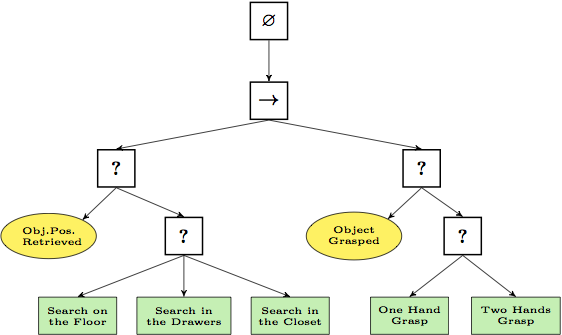
\includegraphics[width=.9\linewidth]{./img/BT_search_and_grasp.png}
\end{column}
\end{columns}
\end{frame}


\begin{frame}[label=sec-2-0-2]{Définition}
\alert{Behaviour tree} (BT):
\begin{itemize}
\item Graphe orienté acyclique
\item Chaque noeud retourne Succès, Échec ou En Cours selon leurs règles associées
\item Évalué par un \emph{tick} qui se propage en profondeur dans le graphe
\end{itemize}

Les noeuds peuvent se trouver sous trois formes, les Composites, les Décorateurs et les noeuds d'Éxécution.
\end{frame}


\begin{frame}[label=sec-2-0-3]{Modularité}
\begin{columns}
\begin{column}{0.5\textwidth}

\begin{itemize}
\item Modulaire: Un BT peu remplacer une feuille
\end{itemize}


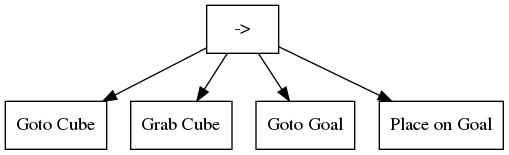
\includegraphics[width=.9\linewidth]{./img/Robot.png}
\end{column}



\begin{column}{0.5\textwidth}

\begin{itemize}
\item Condition: Le BT ne retourne Succès ou Échec
\end{itemize}


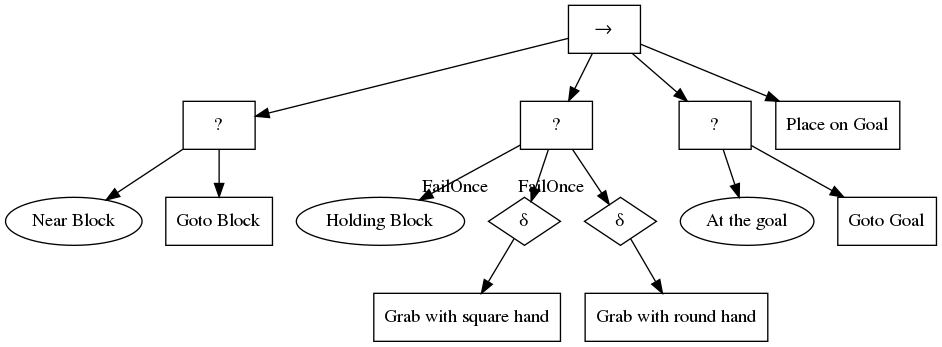
\includegraphics[width=.9\linewidth]{./img/Robot2.png}
\end{column}
\end{columns}
\end{frame}


\begin{frame}[label=sec-2-0-4]{Recherches \& Mission planning}
\begin{columns}
\begin{column}{0.5\textwidth}

\begin{center}
Robotique
\end{center}

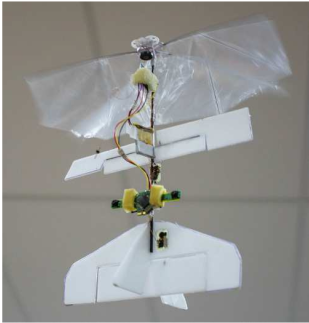
\includegraphics[width=.9\linewidth]{./img/Drone.png}
\end{column}

\begin{column}{0.5\textwidth}

\begin{center}
Jeu vidéo
\end{center}

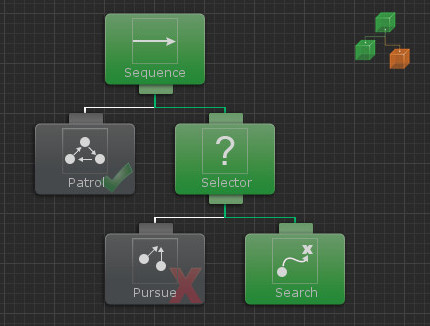
\includegraphics[width=.9\linewidth]{./img/Unity.jpg}
\end{column}
\end{columns}
\end{frame}
\subsection{}
\label{sec-2-1}

\begin{frame}[label=sec-2-1-1]{Noeuds d'éxécution}
\begin{columns}
\begin{column}{0.5\textwidth}

\begin{center}
\alert{Action}
\end{center}

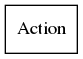
\includegraphics[width=.9\linewidth]{img/Action.png}


Succès si:
Action terminée correctement

Échec si:
Action mal terminée

En Cours si:
Action non terminée
\end{column}


\begin{column}{0.5\textwidth}

\begin{center}
\alert{Condition}
\end{center}

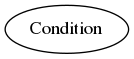
\includegraphics[width=.9\linewidth]{img/Condition.png}


Succès si:
Condition vraie

Échec si:
Condition fausse

En Cours si:
Jamais
\end{column}
\end{columns}
\end{frame}


\begin{frame}[label=sec-2-1-2]{Composites}
\begin{columns}
\begin{column}{0.5\textwidth}

\begin{center}
\alert{Séquence}
\end{center}

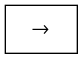
\includegraphics[width=.9\linewidth]{img/Sequence.png}


Succès si:
Tout les enfants ont réussis

Échec si:
Un enfant a échoué

En Cours si:
Un enfant est en cours
\end{column}

\begin{column}{0.5\textwidth}

\begin{center}
\alert{Sélecteur}
\end{center}

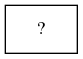
\includegraphics[width=.9\linewidth]{img/Selector.png}


Succès si:
Un enfant a réussi

Échec si:
Tout les enfants ont échoués

En Cours si:
Un enfant est en cours
\end{column}
\end{columns}
\end{frame}

\begin{frame}[label=sec-2-1-3]{Composites}
\begin{columns}
\begin{column}{0.5\textwidth}

\begin{center}
\alert{Parallèle}
\end{center}

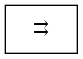
\includegraphics[width=.9\linewidth]{img/Parallel.png}


Succès si:
M enfants ont réussis

Échec si:
F enfants ont échoués

En Cours si:
Aucun des précédents
\end{column}

\begin{column}{0.5\textwidth}

\begin{center}
\alert{Composites avec Mémoire}
\end{center}

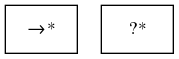
\includegraphics[width=.9\linewidth]{img/Memories.png}

Identique à leurs équivalents sans mémoire.

Mais tant que ce noeud est En Cours, les enfants ayant déjà échoués ou réussis ne sont par re-tickés
\end{column}
\end{columns}
\end{frame}


\begin{frame}[label=sec-2-1-4]{Décorateurs}
\begin{columns}
\begin{column}{0.5\textwidth}

\begin{center}
\alert{Décorateur}
\end{center}

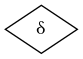
\includegraphics[width=.9\linewidth]{img/Decorateur.png}


Succès, Échec ou En Cours si: 
Personnalisé
\end{column}

\begin{column}{0.5\textwidth}
Exemples:
\begin{itemize}
\item Inverseur
\item Comteur
\item Condition
\end{itemize}
\end{column}
\end{columns}
\end{frame}


\section{BTs \& PacMan}
\label{sec-3}
\begin{frame}[label=sec-3-0-1]{PacMan}
Objectif: Manger tout les PacGums sans se faire manger par les fantômes

\begin{columns}
\begin{column}{0.5\textwidth}

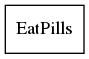
\includegraphics[width=.9\linewidth]{img/EatPills.png}
\end{column}

\begin{column}{0.5\textwidth}

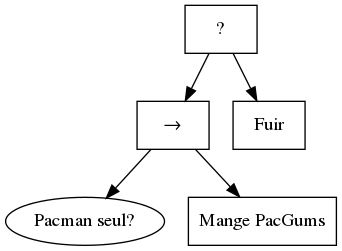
\includegraphics[width=.9\linewidth]{img/EatPills2.png}
\end{column}
\end{columns}
\end{frame}

\begin{frame}[label=sec-3-0-2]{Mouvement déterministe}
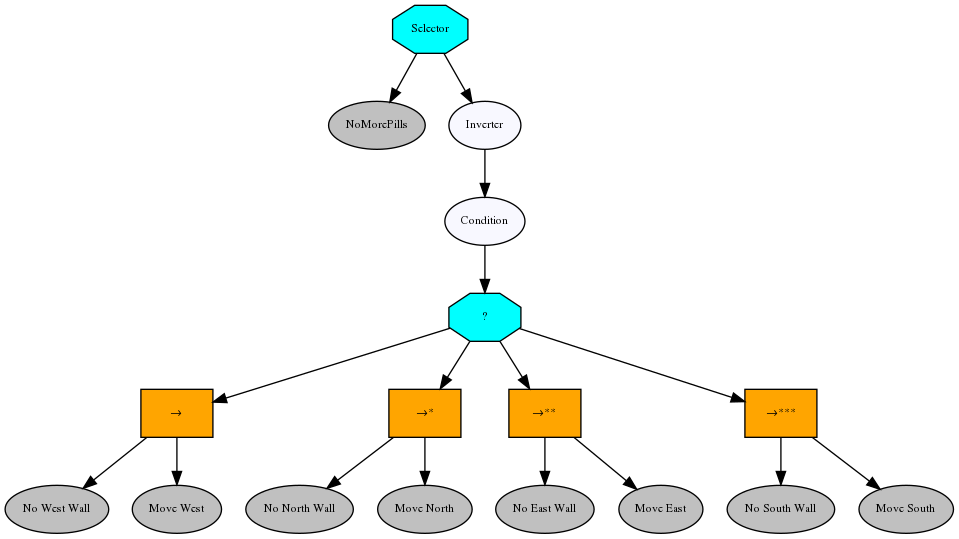
\includegraphics[width=.9\linewidth]{../Archivage/PacMan_v0/PacManDeterministeBT.png}
\end{frame}

\begin{frame}[label=sec-3-0-3]{Mouvement aléatoire}
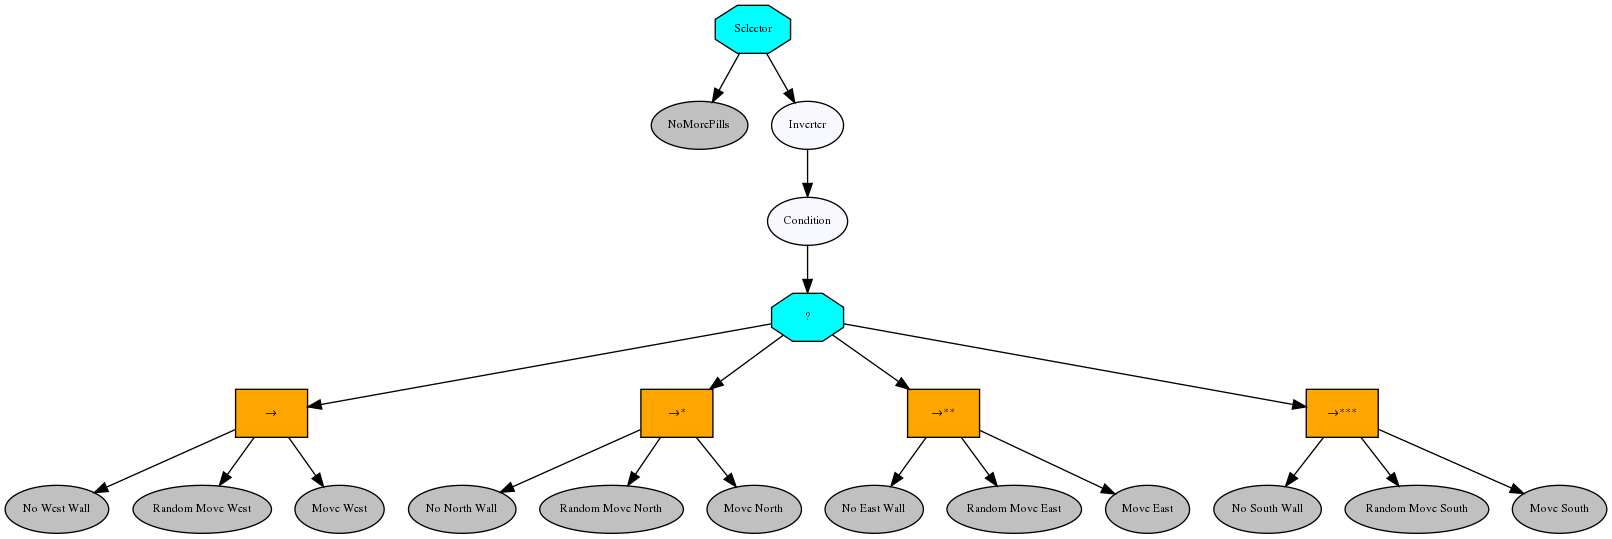
\includegraphics[width=.9\linewidth]{../Archivage/PacMan_v0/PacManRandomBT.png}
\end{frame}

\begin{frame}[label=sec-3-0-4]{Mouvement équiprobable}
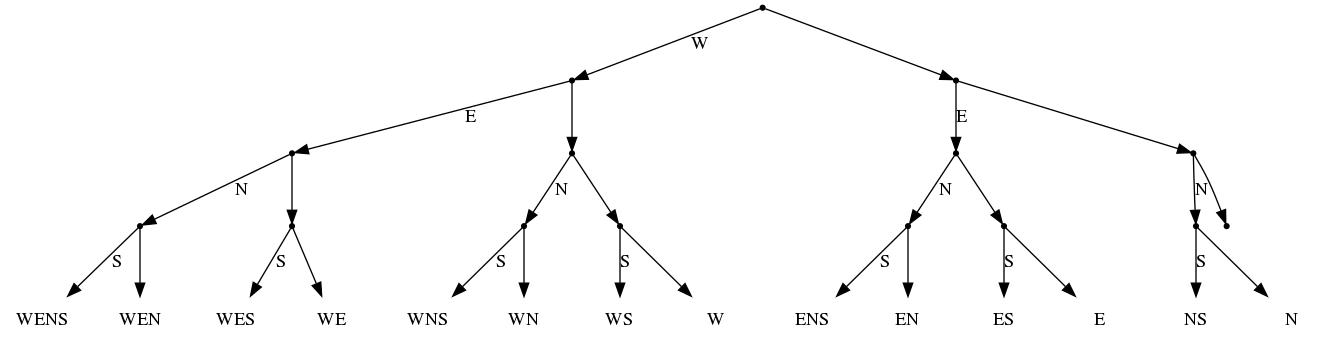
\includegraphics[width=.9\linewidth]{../Archivage/PacMan_v0/SimplifiedEquiprobable.png}
\end{frame}

\begin{frame}[label=sec-3-0-5]{Mouvement équiprobable}
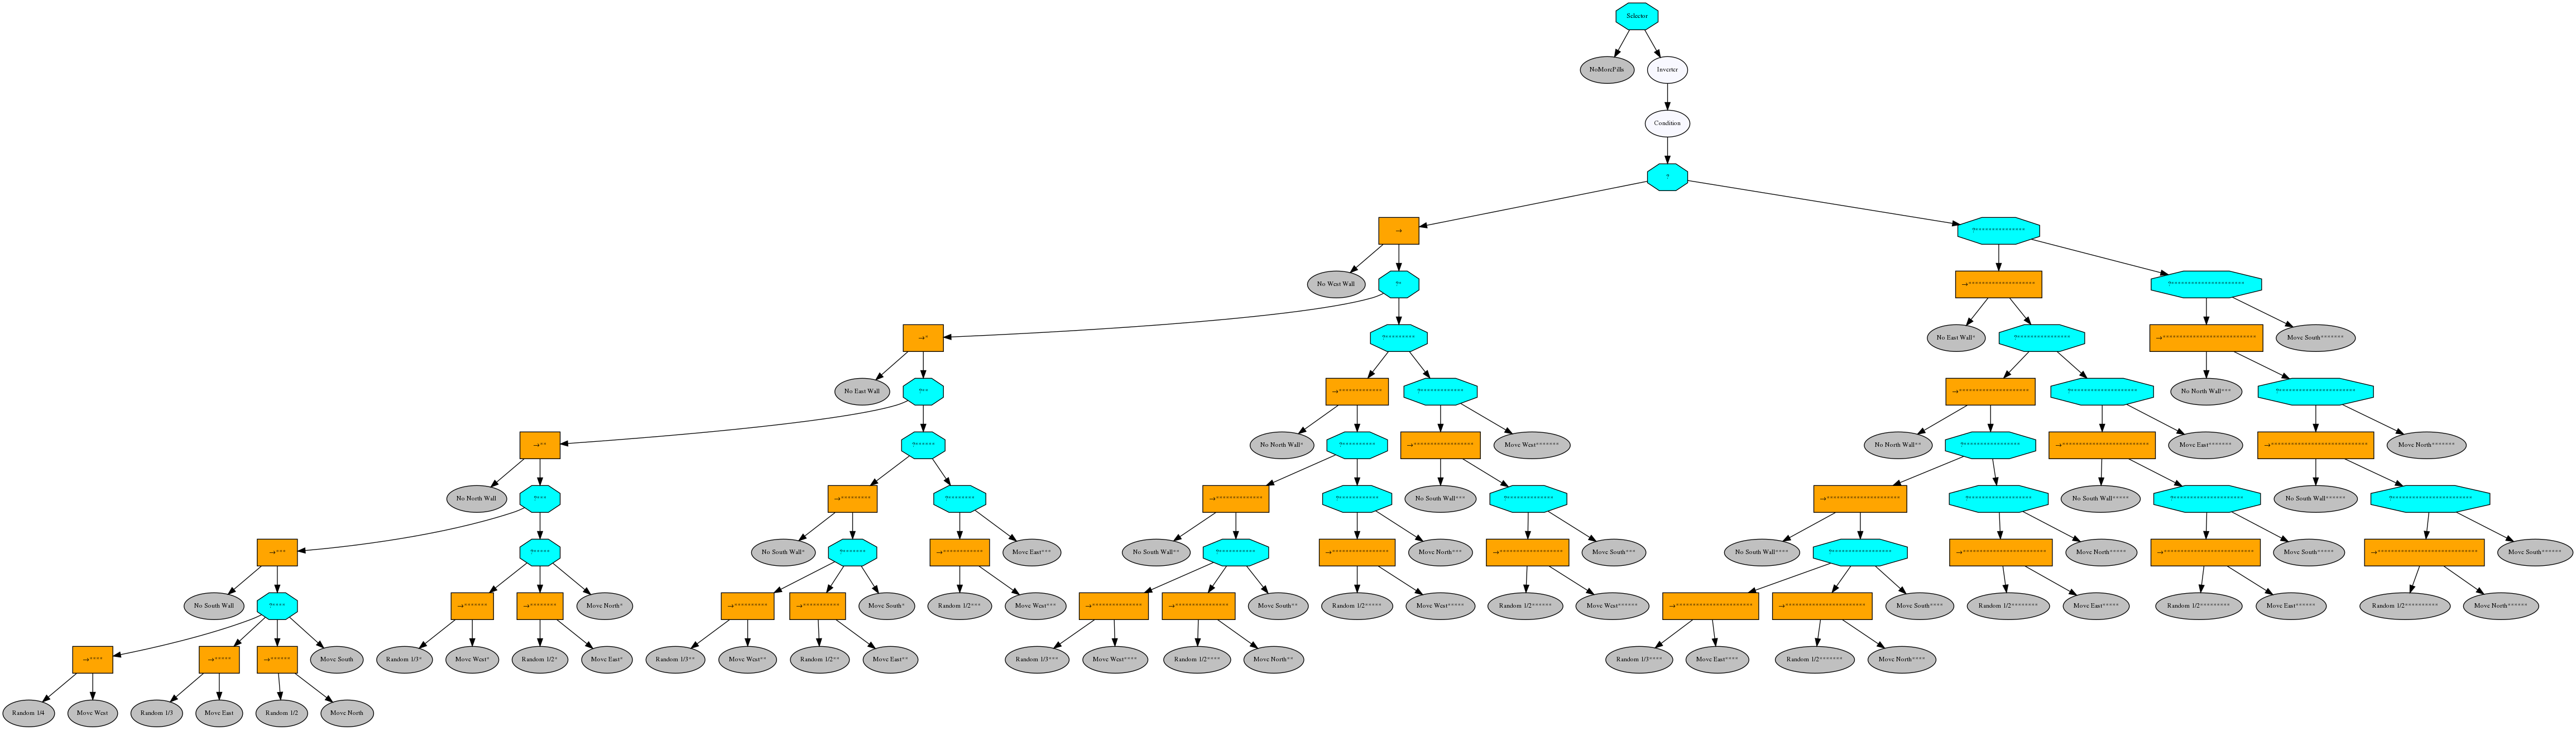
\includegraphics[width=.9\linewidth]{../Archivage/PacMan_v0/PacManEquiprobableBT.png}
\end{frame}

\begin{frame}[label=sec-3-0-6]{Modèle continu}
\begin{center}
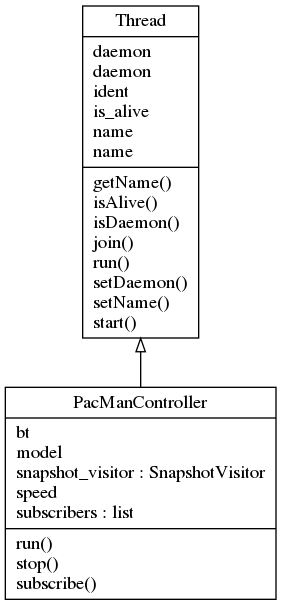
\includegraphics[height=0.68\textwidth]{../WIP/PacMan/classes.png}
\end{center}
\end{frame}

\begin{frame}[label=sec-3-0-7]{Controlleur actuel}
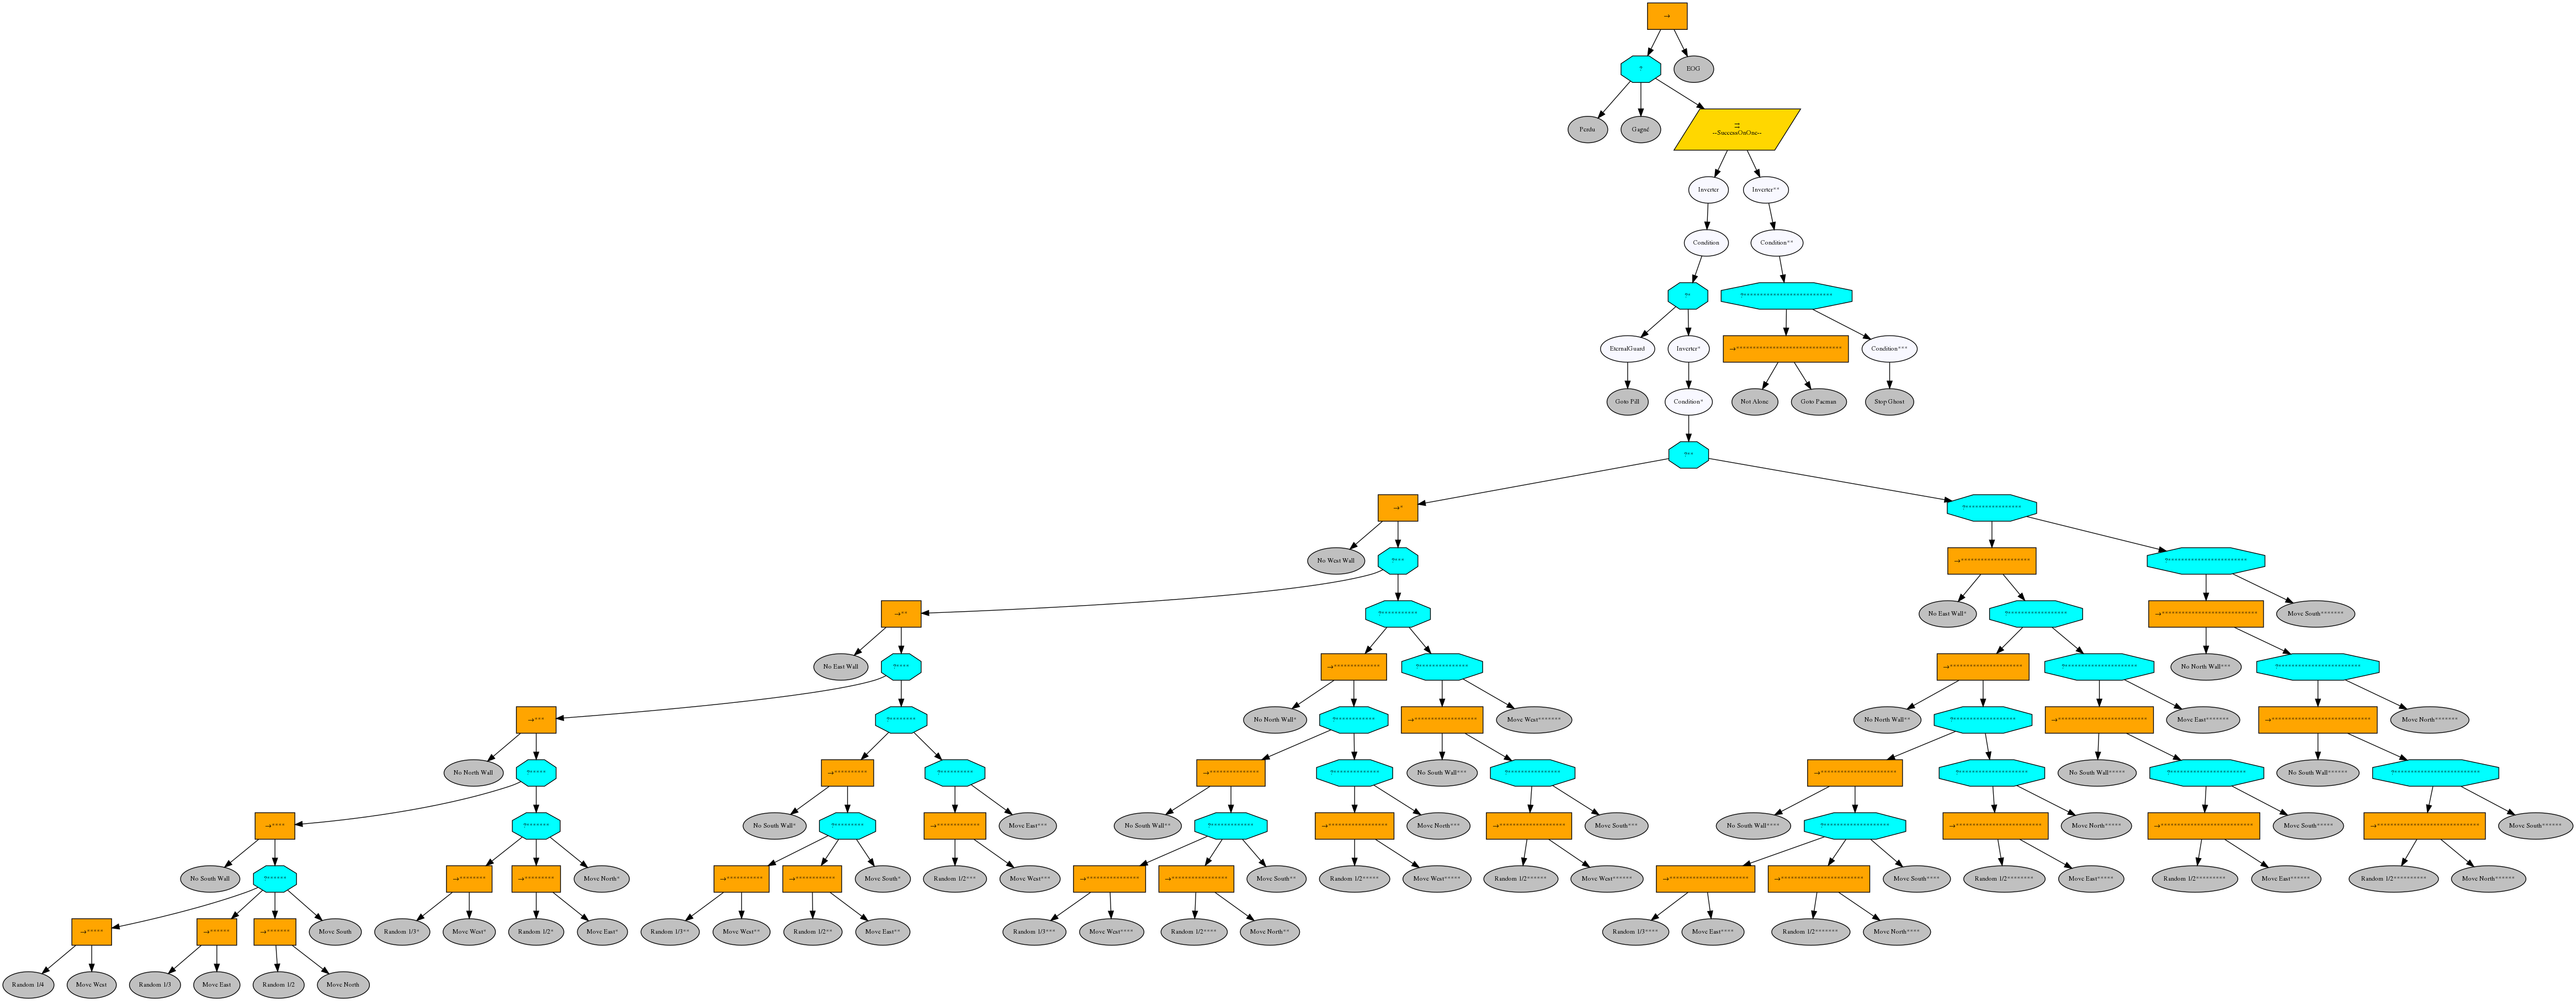
\includegraphics[width=.9\linewidth]{./img/LastPacMan.png}
\end{frame}

\begin{frame}[label=sec-3-0-8]{Rendu}
\begin{center}
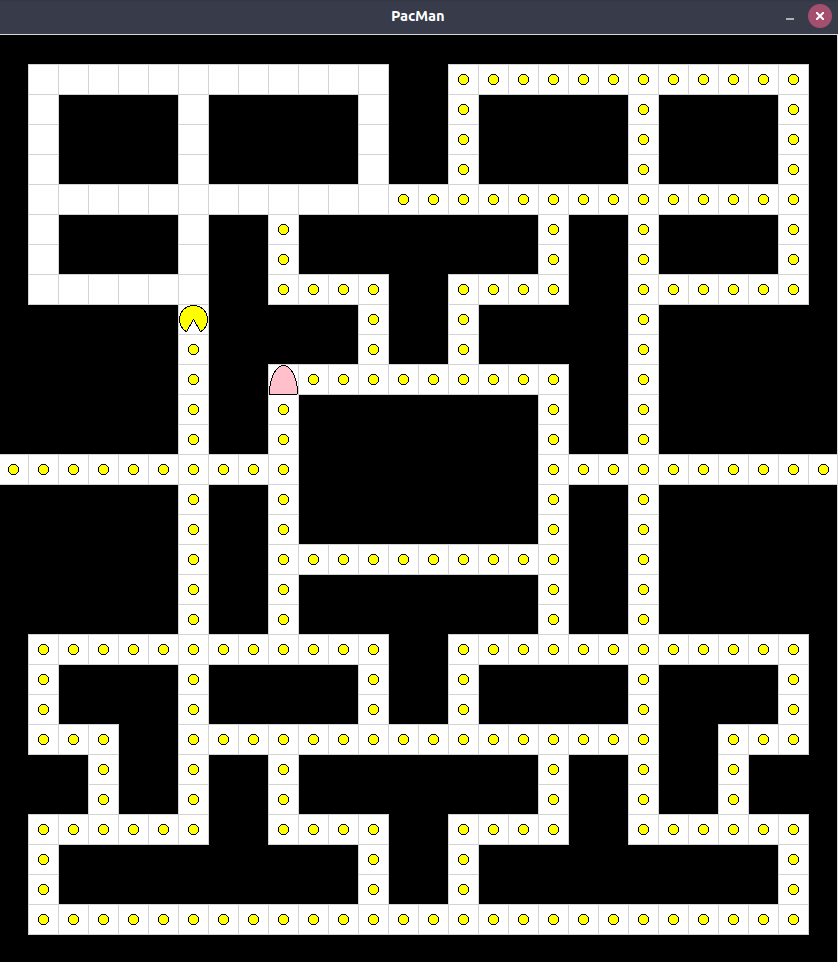
\includegraphics[height=0.68\textwidth]{./img/PacMan.png}
\end{center}
\end{frame}





\section{TPs}
\label{sec-4}
\begin{frame}[label=sec-4-0-1]{TPs}
TP python/POO sur le thème des BTs 

Organisation en 3 TPs:
\begin{itemize}
\item Graphes \& BTs
\item Tkinter
\item Tkinter appliqué au PacMan (MVC)
\end{itemize}
\end{frame}

\section{Conclusion}
\label{sec-5}
\begin{frame}[label=sec-5-0-1]{Conclusion}
\begin{itemize}
\item Modulaire
\item Réactif
\item Intuitif
\end{itemize}
\end{frame}
% Emacs 25.2.2 (Org mode 8.2.10)
\end{document}